\section{Verificación Formal Simbólica con Tamarin Prover}
\label{sec:practica_tamarin}
% =============================================================================

Con el fin de demostrar matemáticamente que la estructura de mensajes del protocolo impide ataques lógicos de suplantación, doble voto o revelación prematura sobre la red, el protocolo fue modelado y verificado mediante la herramienta automatizada \textbf{Tamarin Prover} (versión 1.12.0 junto al motor algebraico Maude 3.5.1 en arquitectura ARM64) bajo el modelo de adversario activo Dolev--Yao.

\subsection{Especificación del Modelo Simbólico y Supuestos}
\label{subsec:tamarin_modelo_formal}

El modelo formal se especificó mediante reglas de reescritura de multiconjuntos de hechos que representan: (1) la teoría ecuacional de encapsulamiento $\text{decaps}(dk, \text{encaps}(\text{ek\_from\_dk}(dk), r)) = r$, cifrado simétrico, firmas digitales y funciones resumen; (2) la generación de claves de las autoridades ($AR$, $SV$ y $AC$); (3) el empadronamiento mediante el hecho lineal de un solo uso $\text{NoHaVotado}(id_V)$, que se consume al votar y se transforma irreversiblemente en el hecho persistente $\text{YaVoto}(id_V)$; (4) el almacenamiento anónimo en la urna $\text{AnforaDigital}(ct_{\text{kem}}, c_{\text{voto}}, ts)$ tras desacoplar la identidad; (5) la apertura y conteo condicionados al hecho de cierre $\text{UrnaCerrada}$; y (6) las reglas de revelación de claves para evaluar qué propiedades se mantienen ante el compromiso de participantes. En la Tabla \ref{tab:supuestos_modelo_tamarin} se resumen los seis supuestos formales del modelo (cuyo código completo se incluye en el Apéndice \ref{anexo:tamarin_spthy}).

\begin{table}[!htbp]
	\centering
	\footnotesize
	\begin{tabularx}{\textwidth}{p{0.6cm}p{2.9cm}X>{\raggedright\arraybackslash}p{4.0cm}}
		\toprule
		\textbf{Id.} & \textbf{Supuesto Declarado} & \textbf{Significado en el Sistema Electoral} & \textbf{Representación en Tamarin} \\
		\midrule
		\textbf{S1} & Autoridades únicas & Opera una sola instancia de AR, AC y SV por elección. & Restricciones de inicialización única. \\
		\textbf{S2} & Clave pública auténtica & El votante recibe la clave auténtica $ek_{\text{AC}}$ antes de cifrar. & Canal autenticado de publicación. \\
		\textbf{S3} & Padrón honesto en SV & El SV verifica el padrón oficial y consume el estado lineal. & Confianza operacional en el padrón. \\
		\textbf{S4} & Cierre temporal único & La urna se cierra una sola vez y bloquea votos tardíos. & Restricción de cierre estricto. \\
		\textbf{S5} & Criptografía ideal & Las primitivas operan como cajas negras perfectas. & Modelo simbólico Dolev--Yao. \\
		\textbf{S6} & Escrutinio fiel en AC & La AC publica los votos descifrados tras cerrarse la urna. & Regla de conteo condicionada al cierre. \\
		\bottomrule
	\end{tabularx}
	\caption{Supuestos declarados del modelo en Tamarin Prover.}
	\label{tab:supuestos_modelo_tamarin}
	\par\vspace{3pt}{\footnotesize\textit{Fuente: Elaboración propia.}}
\end{table}

\subsection{Resultados y Alcance de los Cinco Lemas Demostrados}
\label{subsec:tamarin_resultados}
\label{subsec:tamarin_alcance_lemas}
\label{subsec:tamarin_limites}

Al ejecutar el demostrador automático con derivación de fuentes de tipado sobre 4 núcleos y 8 GB de RAM, Tamarin Prover verificó exitosamente los cinco lemas de seguridad y el lema auxiliar de tipos en un tiempo total de **4,58 segundos**, como detalla la Tabla \ref{tab:resultados_tamarin}.

\begin{table}[!htbp]
	\centering
	\footnotesize
	\begin{tabularx}{\textwidth}{lXccr}
		\toprule
		\textbf{Lema Formal} & \textbf{Propiedad de Seguridad Demostrada} & \textbf{Traza} & \textbf{Resultado} & \textbf{Pasos} \\
		\midrule
		ejecutabilidad & Flujo electoral completo de registro, voto y conteo & $\exists$ & \textbf{Verificado} & 22 \\
		unicidad & Imposibilidad de doble voto por consumo de hecho lineal & $\forall$ & \textbf{Verificado} & 18 \\
		secreto\_voto & Confidencialidad del voto mientras no se filtre $dk_{\text{AC}}$ & $\forall$ & \textbf{Verificado} & 8 \\
		autenticidad\_votante & Toda boleta aceptada proviene de un elector acreditado & $\forall$ & \textbf{Verificado} & 17 \\
		integridad\_voto & Inmutabilidad del voto desde la cabina hasta el conteo & $\forall$ & \textbf{Verificado} & 33 \\
		\midrule
		AUTO\_typing & Lema auxiliar automático de invariante de tipos & $\forall$ & \textbf{Verificado} & 85 \\
		\midrule
		\multicolumn{3}{l}{\textbf{Tiempo total de verificación automática:}} & & \textbf{4,58 s} \\
		\bottomrule
	\end{tabularx}
	\caption{Resultados de la verificación formal en Tamarin.}
	\label{tab:resultados_tamarin}
	\par\vspace{3pt}{\footnotesize\textit{Fuente: Salida oficial de Tamarin Prover 1.12.0 y Maude 3.5.1.}}
\end{table}

\begin{figure}[!htbp]
	\centering
	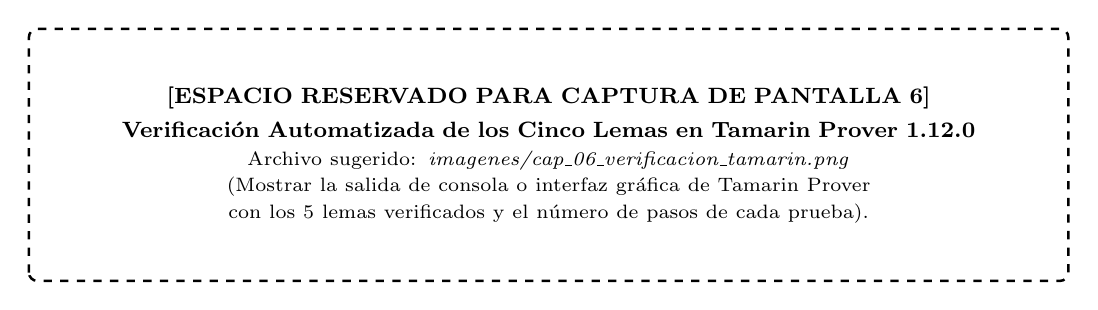
\begin{tikzpicture}
		\draw[line width=0.9pt, dashed, draw=black, fill=white, rounded corners=3pt] (0,0) rectangle (13.2, 3.2);
		\node[align=center, font=\footnotesize\rmfamily, text width=11.8cm] at (6.6, 1.6) {
			\textbf{[ESPACIO RESERVADO PARA CAPTURA DE PANTALLA 6]}\\[3pt]
			\textbf{Verificación Automatizada de los Cinco Lemas en Tamarin Prover 1.12.0}\\[2pt]
			\scriptsize Archivo sugerido: \textit{imagenes/cap\_06\_verificacion\_tamarin.png}\\
			\scriptsize (Mostrar la salida de consola o interfaz gráfica de Tamarin Prover con los 5 lemas verificados y el número de pasos de cada prueba).
		};
	\end{tikzpicture}
	\caption{Verificación formal de lemas en Tamarin Prover.}
	\label{fig:cap_tamarin_prover}
	\par\vspace{2pt}{\footnotesize\textit{Fuente: Elaboración propia.}}
\end{figure}

El lema de \textbf{unicidad} se cumple de forma incondicional gracias al consumo del hecho lineal en el servidor; el \textbf{secreto del voto} se preserva siempre que la clave privada $dk_{\text{AC}}$ de la Autoridad de Conteo no sea filtrada; y los lemas de \textbf{autenticidad} e \textbf{integridad} se sostienen mientras las claves privadas de firma de los electores y de la Autoridad de Registro permanezcan seguras. Como límites declarados del modelo simbólico se dejan registrados la prueba de equivalencia observacional por bi-sistemas (que excede la memoria por explosión de estados), la exclusión de colusión entre servidor y registro (Supuesto S3) y la coacción física presencial fuera del sistema.
